\documentclass[presentation,xcolor={table},9pt]{beamer}

\usepackage{adjustbox}
\usepackage{algorithm}
\usepackage{algpseudocode}
\usepackage{amsfonts}
\usepackage{amsmath}
\usepackage{amssymb}
\usepackage{amsthm}
\usepackage{bookmark}
\usepackage{booktabs}
\usepackage[makeroom]{cancel}
\usepackage[american]{circuitikz}
\usepackage{cite}
% \usepackage{fixmath}
\usepackage[acronym]{glossaries-extra}
\usepackage{hyperref}
\usepackage{import}
\usepackage{mathtools}
\usepackage{microtype}
\usepackage[short]{optidef}
\usepackage{pgfplots}
\usepackage{ragged2e}
\usepackage{siunitx}
\usepackage{stfloats}
\usepackage[caption=false,font=footnotesize,subrefformat=parens,labelformat=parens]{subfig}
\usepackage{tabularx}
\usepackage{tikz}
\usepackage{graphicx}
\usepackage{epstopdf}
\usepackage{multirow}
\usepackage{booktabs}
\usepackage{lastpage}
\usepackage{caption}
\setbeamerfont{caption}{size=\footnotesize}
\captionsetup[figure]{labelformat=empty}
\usefonttheme[onlymath]{serif}

\makeatletter
\@addtoreset{subfigure}{framenumber}
\makeatother

\makeatletter
\newcommand{\forcealgorithm}{\let\@latex@error\@gobble}
\makeatother

% footnote
\newcommand\blfootnote[1]{%
\begingroup
\renewcommand\thefootnote{}\footnote{#1}%
\addtocounter{footnote}{-1}%
\endgroup
}

% amsthm
\newtheorem{proposition}{Proposition}
\newtheorem{remark}{Remark}
% \newtheorem{lemma}{Lemma}
% \newtheorem{corollary}{Corollary}[proposition]

% PGF/TikZ
\pgfplotsset{compat=1.18}
\usepgfplotslibrary{fillbetween,groupplots,patchplots}
\usetikzlibrary{arrows,arrows.meta,automata,backgrounds,calc,math,matrix,patterns,plotmarks,positioning,shapes,angles,quotes}
\usetikzlibrary{decorations.pathmorphing,decorations.pathreplacing,decorations.markings,decorations.shapes,shapes.geometric}

% glossaries-extra
\glsdisablehyper
\setabbreviationstyle[acronym]{long-short}
\newacronym{ai}{AI}{Artificial Intelligence}
\newacronym{af}{AF}{Amplify-and-Forward}
\newacronym{ambc}{AmBC}{Ambient Backscatter Communication}
\newacronym{am}{AM}{Arithmetic Mean}
\newacronym{ao}{AO}{Alternating Optimization}
\newacronym{ap}{AP}{Access Point}
\newacronym{apm}{APM}{Amplitude-Phase Modulation}
\newacronym{awgn}{AWGN}{Additive White Gaussian Noise}
\newacronym{bbc}{BBC}{Bistatic Backscatter Communication}
\newacronym{bcd}{BCD}{Block Coordinate Descent}
\newacronym{bc}{BackCom}{Backscatter Communication}
\newacronym{bd}{BD}{Beyond-Diagonal}
\newacronym{ber}{BER}{Bit Error Rate}
\newacronym{bibo}{BIBO}{Binary-Input Binary-Output}
\newacronym{bls}{BLS}{Backtracking Line Search}
\newacronym{bpcu}{\si{bpcu}}{bits per channel use}
\newacronym{bpsphz}{\si{bps/Hz}}{bits per second per Hertz}
\newacronym{clt}{CLT}{Central Limit Theorem}
\newacronym{cp}{CP}{Canonical Polyadic}
\newacronym{cr}{CR}{Cognitive Radio}
\newacronym{cscg}{CSCG}{Circularly Symmetric Complex Gaussian}
\newacronym{csit}{CSIT}{Channel State Information at the Transmitter}
\newacronym{csi}{CSI}{Channel State Information}
\newacronym{cw}{CW}{Continuous Waveform}
\newacronym{d2d}{D2D}{Device-to-Device}
\newacronym{dcmc}{DCMC}{Discrete-input Continuous-output Memoryless Channel}
\newacronym{dc}{DC}{Direct Current}
\newacronym{df}{DF}{Decode-and-Forward}
\newacronym{dmc}{DMC}{Discrete Memoryless Channel}
\newacronym{dmmac}{DMMAC}{Discrete Memoryless Multiple Access Channel}
\newacronym{dmtc}{DMTC}{Discrete Memoryless Thresholding Channel}
\newacronym{dof}{DoF}{Degree of Freedom}
\newacronym{dp}{DP}{Dynamic Programming}
\newacronym{eirp}{EIRP}{Effective Isotropic Radiated Power}
\newacronym{fdma}{FDMA}{Frequency-Division Multiple Access}
\newacronym{fpga}{FPGA}{Field-Programmable Gate Array}
\newacronym{gm}{GM}{Geomtric Mean}
\newacronym{gp}{GP}{Geometric Programming}
\newacronym{ic}{IC}{Interference Channel}
\newacronym{iid}{i.i.d.}{independent and identically distributed}
\newacronym{im}{IM}{Index Modulation}
\newacronym{ioe}{IoE}{Internet of Everything}
\newacronym{iot}{IoT}{Internet of Things}
\newacronym{kkt}{KKT}{Karush-Kuhn-Tucker}
\newacronym{los}{LoS}{Line-of-Sight}
\newacronym{m2m}{M2M}{Machine-to-Machine}
\newacronym{mac}{MAC}{Multiple Access Channel}
\newacronym{mbc}{MBC}{Monostatic Backscatter Communication}
\newacronym{mc}{MC}{Multiplication Coding}
\newacronym{mimo}{MIMO}{Multiple-Input Multiple-Output}
\newacronym{miso}{MISO}{Multiple-Input Single-Output}
\newacronym{ml}{ML}{Maximum-Likelihood}
\newacronym{mmse}{MMSE}{Minimum Mean-Square-Error}
\newacronym{mrc}{MRC}{Maximal Ratio Combining}
\newacronym{mrt}{MRT}{Maximum Ratio Transmission}
\newacronym{mse}{MSE}{Mean-Square Error}
\newacronym{nlos}{NLoS}{Non-Line-of-Sight}
\newacronym{noma}{NOMA}{Non-Orthogonal Multiple Access}
\newacronym{ofdm}{OFDM}{Orthogonal Frequency-Division Multiplexing}
\newacronym{pc}{PC}{Point-to-point Channel}
\newacronym{pdf}{PDF}{Probability Density Function}
\newacronym{pga}{PGA}{Projected Gradient Ascent}
\newacronym{pin}{PIN}{Positive Intrinsic Negative}
\newacronym{psk}{PSK}{Phase Shift Keying}
\newacronym{ps}{PS}{Power Splitting}
\newacronym{qam}{QAM}{Quadrature Amplitude Modulation}
\newacronym{qos}{QoS}{Quality of Service}
\newacronym{r-e}{R-E}{Rate-Energy}
\newacronym{rcg}{RCG}{Riemannian Conjugate Gradient}
\newacronym{rfid}{RFID}{Radio-Frequency Identification}
\newacronym{rf}{RF}{Radio-Frequency}
\newacronym{ris}{RIS}{Reconfigurable Intelligent Surface}
\newacronym{sca}{SCA}{Successive Convex Approximation}
\newacronym{sc}{SC}{Superposition Coding}
\newacronym{sdma}{SDMA}{Space-Division Multiple Access}
\newacronym{sdp}{SDP}{Semi-Definite Programming}
\newacronym{sdr}{SDR}{Semi-Definite Relaxation}
\newacronym{sic}{SIC}{Successive Interference Cancellation}
\newacronym{simo}{SIMO}{Single-Input Multiple-Output}
\newacronym{sinr}{SINR}{Signal-to-Interference-plus-Noise Ratio}
\newacronym{siso}{SISO}{Single-Input Single-Output}
\newacronym{smawk}{SMAWK}{Shor-Moran-Aggarwal-Wilber-Klawe}
\newacronym{star}{STAR}{Simultaneous Transmission and Reflection}
\newacronym{smf}{SMF}{Scaled Matched Filter}
\newacronym{snr}{SNR}{Signal-to-Noise Ratio}
\newacronym{sr}{SR}{Symbiotic Radio}
\newacronym{svd}{SVD}{Singular Value Decomposition}
\newacronym{swipt}{SWIPT}{Simultaneous Wireless Information and Power Transfer}
\newacronym{tdma}{TDMA}{Time-Division Multiple Access}
\newacronym{ts}{TS}{Time Switching}
\newacronym{ue}{UE}{User Equipment}
\newacronym{wf}{WF}{Water-Filling}
\newacronym{wit}{WIT}{Wireless Information Transfer}
\newacronym{wpcn}{WPCN}{Wireless Powered Communication Network}
\newacronym{wpt}{WPT}{Wireless Power Transfer}
\newacronym{wsn}{WSN}{Wireless Sensor Network}
\newacronym{wsr}{WSR}{Weighted Sum-Rate}
\newacronym{zf}{ZF}{Zero-Forcing}
\newacronym{lc}{LC}{Low-Complexity}
\newacronym{ble}{BLE}{Bluetooth Low Energy}
\newacronym{lora}{LoRa}{Long Range}
\newacronym{lorawan}{LoRaWAN}{Long Range Wide Area Network}
\newacronym{pae}{PAE}{Power-Added Efficiency}
\newacronym{papr}{PAPR}{Peak-to-Average Power Ratio}
\newacronym{fsk}{FSK}{Frequency-Shift Keying}
\newacronym{css}{CSS}{Chirp Spread Spectrum}
\newacronym{dsss}{DSSS}{Direct-Sequence Spread Spectrum}
\newacronym{fsss}{FSSS}{Frequency-Hopping Spread Spectrum}
\newacronym{rz}{RZ}{Return-to-Zero}
\newacronym{nrz}{NRZ}{Non-Return-to-Zero}
\newacronym{leh}{LEH}{Linear Energy Harvester}
\newacronym{fs}{FS}{Frequency-Selective}
\newacronym{rsma}{RSMA}{Rate-Splitting Multiple Access}

\newacronym{embb}{eMBB}{enhanced Mobile Broadband}
\newacronym{urllc}{URLLC}{Ultra-Reliable Low-Latency Communication}
\newacronym{mmtc}{mMTC}{massive Machine-Type Communication}


\usetheme{Frankfurt}
\addtobeamertemplate{navigation symbols}{}{%
    \usebeamerfont{footline}%
    \usebeamercolor[fg]{footline}%
    \hspace{1em}%
	\raisebox{1.5pt}[0pt][0pt]{\insertframenumber/\inserttotalframenumber}
}

\epstopdfsetup{outdir=../assets/viva/}

\title[\glsfmtshort{ris}: Beamforming, Modulation, and Channel Shaping]{\textbf{\glsfmtfull{ris}:\\Beamforming, Modulation, and Channel Shaping}}
\subtitle{Viva Presentation}
\author{Yang Zhao, supervised by Prof Bruno Clerckx}
\institute{Department of Electrical and Electronic Engineering\\Imperial College London}
% \date{\today}
\date{May 2, 2024}

\begin{document}

\frame{\titlepage}


\begin{section}{Intro}
	\begin{frame}{Do we want more waves in the air?}
		\begin{block}{Massive \glsfmtshort{mimo} is here}
			\begin{figure}
				\centering
				\subfloat[8T8R and m\glsfmtshort{mimo} at Imperial]{
					\resizebox{!}{3cm}{
						\includegraphics{../assets/viva/massive_mimo.jpg}
					}
				}
				\subfloat[Cellular statistics]{
					\resizebox{!}{3cm}{
						\includegraphics{../assets/viva/cellular_analysis.png}
					}
				}
			\end{figure}
		\end{block}
		\begin{block}{How far are we from the Shannon capacity?}
			\begin{equation*}
				C(\mathbf{H}) = \max_{\mathbf{Q} \succeq 0, \mathrm{tr}(\mathbf{Q}) \le P} \log \det \left( \mathbf{I} + \rho \mathbf{H} \mathbf{Q} \mathbf{H}^\mathsf{H} \right)
			\end{equation*}
			\vspace{-1em}
			\begin{itemize}
				\item Modulation, coding, and beamforming to \textcolor{gray}{adapt to} the stochastic channel
				\item \gls{ris} can \textcolor{blue}{shape and control} the channel
			\end{itemize}
		\end{block}
	\end{frame}

	\begin{frame}{What is \glsfmtshort{ris}?}
		A planar surface of controllable scattering elements for signal amplitude and phase manipulation \cite{Wu2020}.
		\begin{figure}
			\centering
			\includegraphics[width=0.65\textwidth]{../assets/viva/ris_architecture.pdf}
			\label{fg:ris_architecture}
		\end{figure}
		\begin{block}{Characteristics}
			\begin{itemize}
				\item Low-power and low-cost
				\item Negligible noise and latency
				\item Full-duplex without self-interference
				\item Programmable in real-time
			\end{itemize}
		\end{block}
	\end{frame}

	\begin{frame}{Ancestor of \glsfmtshort{ris}: Reflectarray antenna}
		% not parabolic with parallel phase front
		A reflectarray antenna consists of an array illuminated by a feeding antenna \cite{Deng2016}.
		\begin{figure}
			\centering
			\includegraphics[width=0.45\textwidth]{../assets/viva/reflectarray.png}
		\end{figure}
		A progressive phase shift can be applied to the unit cells (a.k.a. elements) to steer the beam direction.
	\end{frame}

	\begin{frame}{What is the difference in \glsfmtshort{ris}?}
		\begin{enumerate}
			\item Metamaterial enables \textcolor{blue}{real-time control} and \textcolor{blue}{unconventional bahavior}.
			\item Impinging waves can be \textcolor{blue}{partially refracted and reflected}.
			\item The feed can be \textcolor{blue}{mobile} while the surface is \textcolor{blue}{scalable and multi-functional}.
			\item Elements can be physically interconnected for \textcolor{blue}{cooperative wave scattering}.
		\end{enumerate}
		\begin{exampleblock}{Refraction}
			\begin{columns}[T]
				\begin{column}{.25\textwidth}
					\begin{figure}
						\centering
						\resizebox{\columnwidth}{!}{
							\input{../assets/viva/nim_focus.tex}
						}
					\end{figure}
				\end{column}
				% \hfill
				\begin{column}{.6\textwidth}
					\vspace{0.5cm}
					\begin{itemize}
						\item Negative index material can focus waves
						\item Amplitude and phase responses can be tuned by diodes and \glsfmtshort{fpga}
						\item Similar for wave reflection
					\end{itemize}
				\end{column}
			\end{columns}
		\end{exampleblock}
		\begin{exampleblock}{Reflection}
			\vspace{-1cm}
			\begin{figure}[H]
				\centering
				\subfloat[Incident wave\label{fg:wave_incident}]{
					\resizebox{!}{2.02cm}{
						\input{../assets/viva/wave_incident.tex}
					}
				}
				\subfloat[Reflected wave\label{fg:wave_reflected}]{
					\resizebox{!}{2cm}{
						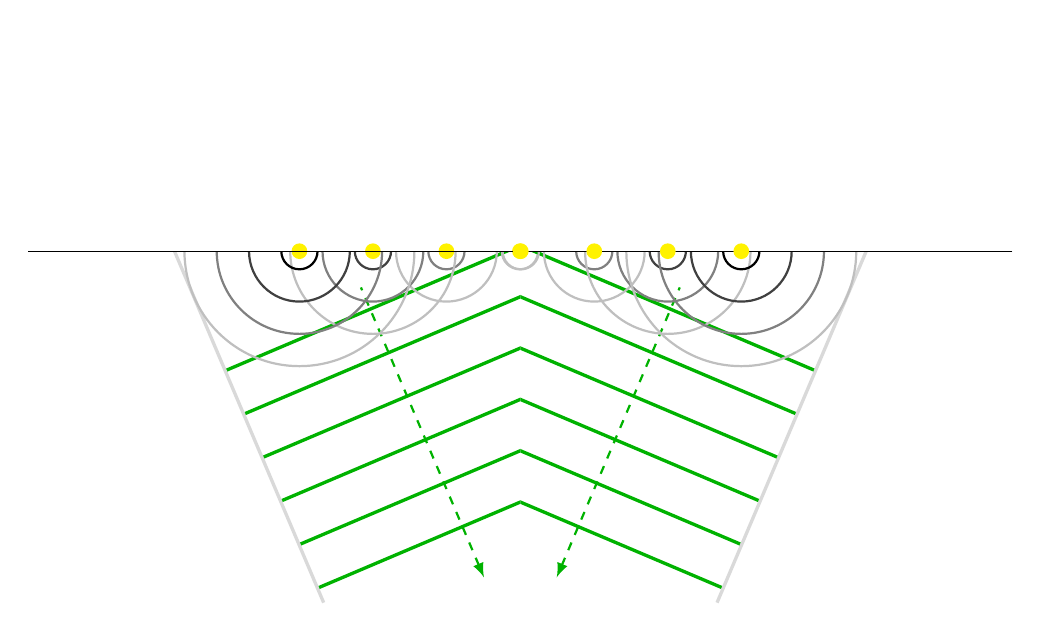
\begin{tikzpicture}[pics/v/.style={code={\draw (0,-#1) -- (0,#1);}}]
	\begin{scope}
		\clip[overlay] (-5,-5) rectangle (5,0);
		\path[rotate=140,overlay=false,very thick]
		foreach \x in {0,...,9}
			{(-2,-2+0.6*\x) coordinate (L\x) edge[blue,opacity=0,name path global=p\x] ++ (4,0) coordinate (R\x)};
	\end{scope}
	\begin{scope}[xshift=-0.97cm]
		\clip[overlay] (-5,0) rectangle (2.22,-5);
		\pgfmathsetmacro{\myx}{2*cos(30)/cos(30)}
		\path[rotate=203,overlay=false,very thick]
		foreach \x in {0,...,5}
			{(-\myx,0.8+0.6*\x) coordinate (L-\x) edge[green!70!black] ++ (2*\myx,0) coordinate (R-\x)}
		%    (-\myx,-2) edge[gray!30] ++(0,6)
		(\myx,-2) edge[gray!30] ++(0,6)
		%    (0,-2) edge[gray!30] ++(0,7)
		(0,4.5) edge[green!70!black,thick,dashed,latex-] ++ (0,-4);
	\end{scope}
	\path[name path=h] (-5,0) coordinate (L) -- (5,0) coordinate (R);
	\foreach \x in {2,3,4,5}
		{\path[name intersections={of=h and p\x,by=i\x}] (i\x);
			\foreach \y in {1,...,\the\numexpr\x-1}
				{
					\pgfmathtruncatemacro{\myf}{50*(\x-\y)}
					\draw[thick,gray!\myf] (i\x) ++ (-0.18+\y*0.41,0)
					arc[start angle=0,end angle=-180,radius=-0.18+0.41*\y];}}
	\draw (L) -- (R);
	\path foreach \x in {2,3,4,5} {(i\x) node[circle,fill,yellow,inner sep=2pt]{}};

	\begin{scope}[xscale=-1,xshift=-2.5cm]
		\begin{scope}
			\clip[overlay] (-5,-5) rectangle (5,0);
			\path[rotate=140,overlay=false,very thick]
			foreach \x in {0,...,9}
				{(-2,-2+0.6*\x) coordinate (L\x) edge[blue,opacity=0,name path global=p\x] ++ (4,0) coordinate (R\x)};
		\end{scope}
		\begin{scope}[xshift=-0.97cm]
			\clip[overlay] (-5,0) rectangle (2.22,-5);
			\pgfmathsetmacro{\myx}{2*cos(30)/cos(30)}
			\path[rotate=203,overlay=false,very thick]
			foreach \x in {0,...,5}
				{(-\myx,0.8+0.6*\x) coordinate (L-\x) edge[green!70!black] ++ (2*\myx,0) coordinate (R-\x)}
			%    (-\myx,-2) edge[gray!30] ++(0,6)
			(\myx,-2) edge[gray!30] ++(0,6)
			%    (0,-2) edge[gray!30] ++(0,7)
			(0,4.5) edge[green!70!black,thick,dashed,latex-] ++ (0,-4);
		\end{scope}
		\path[name path=h] (-5,0) coordinate (L) -- (5,0) coordinate (R);
		\foreach \x in {2,3,4,5}
			{\path[name intersections={of=h and p\x,by=i\x}] (i\x);
				\foreach \y in {1,...,\the\numexpr\x-1}
					{
						\pgfmathtruncatemacro{\myf}{50*(\x-\y)}
						\draw[thick,gray!\myf] (i\x) ++ (-0.18+\y*0.41,0)
						arc[start angle=0,end angle=-180,radius=-0.18+0.41*\y];}}
		\draw (L) -- (R);
		\path foreach \x in {2,3,4,5} {(i\x) node[circle,fill,yellow,inner sep=2pt]{}};
	\end{scope}

\end{tikzpicture}

					}
				}
			\end{figure}
		\end{exampleblock}
	\end{frame}

	\begin{frame}{Use case: Beamforming}
		% \textcolor{blue}{Joint beamforming} design of \gls{ris} and transceiver for a specific performance measure \cite{Wu2020}.
		% \gls{ris} and transceiver \textcolor{blue}{joint beamforming} design for a specific performance measure \cite{Wu2020}.
		\textcolor{blue}{Beamforming} of \gls{ris} and transceiver can be jointly designed for a specific performance measure \cite{Wu2020}.
		\begin{figure}
			\centering
			\subfloat[Coverage extension]{
				\resizebox{!}{2.75cm}{
					\includegraphics{../assets/viva/ris_beamforming_coverage.jpg}
				}
			}
			\subfloat[Security enhancement]{
				\resizebox{!}{2.75cm}{
					\includegraphics{../assets/viva/ris_beamforming_security.jpg}
				}
			}
			\subfloat[Interference mitigation]{
				\resizebox{!}{2.75cm}{
					\includegraphics{../assets/viva/ris_beamforming_interference.jpg}
				}
			}
			\\
			\subfloat[Assist \glsfmtshort{d2d} network]{
				\resizebox{!}{2.75cm}{
					\includegraphics{../assets/viva/ris_beamforming_network.jpg}
				}
			}
			\subfloat[Assist information and power transfer]{
				\resizebox{!}{2.75cm}{
					\includegraphics{../assets/viva/ris_beamforming_swipt.jpg}
				}
			}
		\end{figure}
	\end{frame}

	\begin{frame}{Use case: Modulation}
		\gls{ris} can be used for backscatter \textcolor{blue}{modulation} by periodically switching the reflection pattern \cite{Hu2021a}.
		\begin{figure}
			\centering
			\includegraphics[width=0.9\textwidth]{../assets/viva/ris_modulation.pdf}
		\end{figure}
	\end{frame}

	\begin{frame}{Use case: Channel shaping}
		\textcolor{blue}{Channel shaping} exploits the \gls{ris} as a stand-alone device to modify the inherent properties of the propagation environment \cite{Arslan2022}.
		\begin{figure}
			\centering
			\includegraphics[width=0.9\textwidth]{../assets/viva/ris_shaping.pdf}
		\end{figure}
	\end{frame}
\end{section}

\begin{section}{Beamforming: \glsfmtshort{ris}-Aided \glsfmtshort{swipt}}
	\begin{frame}{\glsfmtshort{ris}-aided \glsfmtshort{swipt}: Joint waveform and beamforming design}
		\begin{block}{Overview}
			\begin{itemize}\setlength\itemsep{20pt}
				\item \textit{What does this paper propose?}

				A single-user multi-carrier \gls{swipt} system aided by a passive \gls{ris}.
				\item \textit{How does it differ from previous work?}

				We consider waveform and beamforming design for practical receiver architectures under non-linear harvester and frequency-flat \gls{ris} models.
				\item \textit{What are the benefits?}

				It exploits the spatial-frequency domain and rectifier behavior to enlarge the \gls{r-e} region, achieving squared asymptotic performance than conventional designs.
			\end{itemize}
		\end{block}
	\end{frame}

	\begin{frame}{\glsfmtshort{wpt} via radio waves}
		\vspace{-0.5cm}
		\begin{table}
			\footnotesize
			\rowcolors{2}{gray!25}{white}
			\renewcommand{\arraystretch}{1.25}
			\resizebox{\linewidth}{!}{
				\begin{tabular}{c c c c c c}
					\toprule
					% \hiderowcolors
					Categories                   & Medium                     & Device                     & Power level                            & Frequency                                & Range                     \\ \midrule
					% \showrowcolors
					                             & Magnetic resonant coupling & Resonators                 & Up to \SI{10}{\W}                      & \si{\kHz} -- \si{\MHz}                   & \si{\m}                   \\
					\cellcolor{white}            & Inductive coupling         & Wire coils                 & Up to \SI{10}{\W}                      & \si{\Hz} -- \si{\MHz}                    & \si{\cm}                  \\
					\multirow{-3}{*}{Near-field} & Capacitive coupling        & Metal plates               & Up to \SI{1}{\W}                       & \si{\kHz} -- \si{\MHz}                   & \si{\mm}                  \\
					\cellcolor{white}            & \textcolor{blue}{\gls{rf} wave}  & \textcolor{blue}{Rectenna} & \textcolor{blue}{\si{\uW} -- \si{\mW}} & \textcolor{blue}{\si{\MHz} -- \si{\GHz}} & \textcolor{blue}{\si{\m}} \\
					\multirow{-2}{*}{Far-field}  & Light wave                 & Laser                      & \si{\uW} -- \si{\mW}                   & \si{\THz}                                & \si{\km}                  \\ \bottomrule
				\end{tabular}
			}
		\end{table}
		\vspace{-0.25cm}
		\begin{figure}[H]
			\centering
			\resizebox{\columnwidth}{!}{
				\begin{circuitikz}[transform shape,align=center,font=\footnotesize]
	\draw(0,0) node[draw](rf){\gls{rf}\\source};
	\draw(rf.east) node[txantenna]{};
	\draw(1,1) node{Tx};
	\draw(4.875,2) node[draw]{\gls{ris}};
	\draw(4.875,1) node[draw]{Channel};
	\draw(10,0) node[draw](mc){Matching\\network};
	\draw(mc.west) node[rxantenna,xscale=-1]{};
	\draw(8.7,1) node{Rx};
	\draw(mc.east) to ++(0.85,0) node[anchor=west,draw](d){Diode};
	\draw(d.east) to ++(0.85,0) node[anchor=west,draw](lpf){Low-pass\\filter};
	\draw(lpf.east) to ++(1,0) node[anchor=west,draw](dd){\gls{dc}-\gls{dc}\\converter};
	\draw(dd.east) to ++(1,0) node[anchor=west,draw](s){Storage};

	\draw [dashed] (-0.95,-0.75) rectangle (3.75,2.75);
	\draw (1.4,3) node[]{Energy transmitter};
	\draw [dotted] (6.25,-0.5) rectangle (15.6,2.5);
	\draw (10.925,2) node[]{Rectenna};
	\draw [dotted] (16,-0.5) rectangle (20.5,1.25);
	\draw (18.25,0.875) node[]{Power management unit};
	\draw [dashed] (6,-0.75) rectangle (20.75,2.75);
	\draw (13.375,3) node[]{Energy receiver};

	\draw (-0.95,-1) node[]{$P_{\mathrm{DC}}^{\mathrm{T}}$};
	\draw (3.75,-1) node[]{$P_{\mathrm{RF}}^{\mathrm{T}}$};
	\draw (6,-1) node[]{$P_{\mathrm{RF}}^{\mathrm{R}}$};
	\draw (15.8,-1) node[]{$P_{\mathrm{DC}}^{\mathrm{R}}$};
	\draw (20.5,-1) node[]{$P_{\mathrm{DC}}^{\mathrm{S}}$};

	\draw[gray,dashdotted,-latex] (10.925,-0.5) to ++(0,-1.5) to ++(-1,0) node[anchor=east,draw](c){Channel\\feedback};
	\draw[gray,dashdotted,latex-] (1.4,-0.75) to ++(0,-1.25) to ++(1,0) node[anchor=west,draw](s){Signal\\optimization};
	\draw[gray,dashdotted,-latex] (c.west) to (s.east);
	\draw[gray] (6.45,-2) node[]{Reverse\\communication link};
\end{circuitikz}

			}
			\label{fg:wpt_architecture}
		\end{figure}
		\vspace{-1em}
		The end-to-end \gls{wpt} efficiency is
		\begin{equation*}
			\eta = \frac{P_{\mathrm{DC}}^\mathrm{S}}{P_{\mathrm{DC}}^\mathrm{T}} = \underbrace{\frac{P_{\mathrm{RF}}^\mathrm{T}}{P_{\mathrm{DC}}^\mathrm{T}}}_{\eta_1} \textcolor{orange}{\underbrace{\frac{P_{\mathrm{RF}}^\mathrm{R}}{P_{\mathrm{RF}}^\mathrm{T}}}_{\eta_2}} \textcolor{blue}{\underbrace{\frac{P_{\mathrm{DC}}^\mathrm{R}}{P_{\mathrm{RF}}^\mathrm{R}}}_{\eta_3}} \underbrace{\frac{P_{\mathrm{DC}}^\mathrm{S}}{P_{\mathrm{DC}}^\mathrm{R}}}_{\eta_4}
		\end{equation*}
		where $\eta_2$ and $\eta_3$ models the channel and rectenna, respectively.
	\end{frame}

	\begin{frame}{Received signal and harvested power}
		The rectenna efficiency $\eta_3$ depends on its input waveform (power and shape).
		\begin{block}{Rectenna model}
			% \vspace{-0.25cm}
			% \begin{figure}[H]
			% 	\centering
			% 	\subfloat[Rectenna]{
			% 		\resizebox{0.35\columnwidth}{!}{
			% 			\input{../assets/viva/rectenna.tex}
			% 		}
			% 		\label{fg:rectenna}
			% 	}
			% 	\subfloat[Half-wave rectifier]{
			% 		\resizebox{0.35\columnwidth}{!}{
			% 			\input{../assets/viva/halfwave_rectifier.tex}
			% 		}
			% 		\label{fg:halfwave_rectifier}
			% 	}
			% \end{figure}
			% \vspace{-0.25cm}
			\begin{itemize}
				\item Linear region (constant $\eta_3$): $P_{\mathrm{DC}}^\mathrm{R} = \eta_3 P_\mathrm{RF}^\mathrm{R} = \eta_3 \mathbb{A}\bigl\{ \lvert y(t) \rvert^2 \bigr\}$
				\item Non-linear region: Taylor expansion on diode characteristic equation
				\vspace{-0.25cm}
				\begin{equation*}
					\arg_{x(t)} \max P_{\mathrm{DC}}^\mathrm{R} = \arg_{x(t)} \max z \triangleq \sum_{i=2,\text{even}}^{n_0} \beta_i \mathbb{A}\bigl\{ y^i(t) \bigr\},
					\vspace{-0.5cm}
				\end{equation*}
				where $\beta_i = I_\mathrm{S} \frac{R_\mathrm{A}^{i/2}}{i!(n v_\mathrm{T})^i}$ is a constant and $n_0$ is the truncation order.
			\end{itemize}
		\end{block}
		\begin{alertblock}{In multi-carrier \glsfmtshort{wpt} \textellipsis}
			\begin{itemize}
				\item $n_0 \ge 4$ allows components to compensate each other for higher \gls{dc} power
				\item High \gls{papr} (e.g., multi-sine) is preferred \cite{Trotter2009}
			\end{itemize}
			\vspace{-0.5cm}
			\begin{figure}
				\centering
				\subfloat{
					\resizebox{!}{2.5cm}{
						\includegraphics{../assets/viva/multisine_frequency_domain.eps}
					}
				}
				\subfloat{
					\resizebox{!}{2.5cm}{
						\includegraphics{../assets/viva/multisine_time_domain.eps}
					}
				}
			\end{figure}
		\end{alertblock}
	\end{frame}

	\begin{frame}{From \glsfmtshort{wpt} to \gls{ris}-aided \glsfmtshort{swipt}}
		\begin{figure}[H]
			\centering
			\def\svgwidth{0.5\columnwidth}
			\input{../assets/viva/system.eps_tex}
		\end{figure}

		\begin{itemize}
			\item \gls{swipt} features shared signal, spectrum, and infrastructure
			\item \gls{ris} enhances the RF-to-RF efficiency $\eta_2$ which has been a major concern
		\end{itemize}
		\begin{block}{Transmit waveform}
			\begin{equation*}
				\mathbf{x}(t) = \Re \left\{\sum_{n=1}^N \Bigl(\mathbf{w}_{\mathrm{I},n} \cdot \underbrace{\tilde{x}_{\mathrm{I},n}(t) e^{\jmath 2{\pi}{f_n}{t}}}_\text{modulated}+\mathbf{w}_{\mathrm{P},n} \cdot \underbrace{e^{\jmath 2{\pi}{f_n}{t}}}_\text{multi-sine}\Bigr) \right\}
			\end{equation*}
		\end{block}
		\begin{block}{Frequency-flat \glsfmtshort{ris} model}
			\begin{equation*}
				\mathbf{h}_{n}^\mathsf{H} = \mathbf{h}_{\mathrm{D},n}^\mathsf{H} + \mathbf{h}_{\mathrm{B},n}^\mathsf{H} \mathbf{\Theta} \mathbf{H}_{\mathrm{F},n}
			\end{equation*}
		\end{block}
	\end{frame}

	\begin{frame}{Performance analysis}
		\begin{block}{Receiver architectures}
			\vspace{-0.5cm}
			\begin{figure}
				\centering
				\subfloat[\gls{ts} receiver]{
					\resizebox{0.48\columnwidth}{!}{
						\begin{circuitikz}[transform shape,align=center]
	\draw (0,0) node[bareRXantenna](r){Rx}(r.center)
		to[short] ++(0,-1) node[below]{Time switcher}
		to[short] node[spdt,anchor=in](s){} ++(0.5,0);

	\draw (s.out 1)
		to ++(1.25,0)
		to ++(0,0.5)
		to ++(1,0) node[draw,minimum width=2.5cm,anchor=west](eh){Energy\\harvester};
	% \draw (eh.east) to ++(1,0) node[draw,anchor=west,minimum width=2.5cm]{Power\\management};

	\draw (s.out 2)
		to ++(1.25,0)
		to ++(0,-0.5)
		to ++(1,0) node[draw,anchor=west,minimum width=2.5cm]{Information\\decoder};
\end{circuitikz}

% \begin{circuitikz}[transform shape,align=center]
% 	\draw (0,0) node[bareRXantenna](r){Rx}(r.center)
% 		to[short] ++(0,-1)
% 		to node[coupler,anchor=left up](c){Power splitter} ++(1,0);
% 	\draw (c.right up)
% 		to[short] ++(0.5,0)
% 		to ++(0,0.5)
% 		to ++(1,0) node[draw,minimum width=2.5cm,anchor=west](eh){Energy\\harvester};
% 	\draw (eh.east) to ++(1,0) node[draw,anchor=west,minimum width=2.5cm]{Power\\management};
% 	\draw (c.right down)
% 		to[short] ++(0.5,0)
% 		to ++(0,-0.5)
% 		to ++(1,0) node[draw,anchor=west,minimum width=2.5cm]{Information\\decoder};
% \end{circuitikz}

					}
					\label{fg:receiver_ts}
				}
				\subfloat[\gls{ps} receiver]{
					\resizebox{0.48\columnwidth}{!}{
						\begin{circuitikz}[transform shape,align=center]
	\draw (0,0) node[bareRXantenna](r){Rx}(r.center)
		to[short] ++(0,-1)
		to node[coupler,anchor=left up](c){Power splitter} ++(1,0);
	\draw (c.right up)
		to[short] ++(0.5,0)
		to ++(0,0.5)
		to ++(1,0) node[draw,minimum width=2.5cm,anchor=west](eh){Energy\\harvester};
	% \draw (eh.east) to ++(1,0) node[draw,anchor=west,minimum width=2.5cm]{Power\\management};
	\draw (c.right down)
		to[short] ++(0.5,0)
		to ++(0,-0.5)
		to ++(1,0) node[draw,anchor=west,minimum width=2.5cm]{Information\\decoder};
\end{circuitikz}

					}
					\label{fg:receiver_ps}
				}
			\end{figure}
		\end{block}
		\begin{block}{\glsfmtfull{r-e} region of \glsfmtshort{ps}}
			\vspace{-0.25cm}
			\begin{align*}
				R(\boldsymbol{\theta},\mathbf{w}_{\mathrm{I}},\rho) &= \sum_{n=1}^N{\log_2\left(1+\frac{(1-\rho)\lvert \mathbf{h}_{n}^\mathsf{H}\mathbf{w}_{\mathrm{I},n} \rvert^2}{\sigma_n^2}\right)},\\
				z(\boldsymbol{\theta},\mathbf{w}_{\mathrm{I}},\mathbf{w}_{\mathrm{P}},\rho) &= \sum_{i=2,\text{even}}^{n_0}{\beta_i}{\rho^{i/2}}{\mathbb{E}\left\{\mathbb{A}\left\{y^i(t)\right\}\right\}},
			\end{align*}
			\begin{equation*}
				\mathcal{C}_\mathrm{R-E}(P)\triangleq \Bigl\{(r,e) : 0 \le r \le R, \ 0 \le e \le z, \lVert{\mathbf{W}_{\mathrm{I}}}\rVert _\mathrm{F}^2/2 + \lVert{\mathbf{W}_{\mathrm{P}}}\rVert _\mathrm{F}^2/2 \le P \Bigr\}
			\end{equation*}
		\end{block}
	\end{frame}

	\begin{frame}{Joint waveform and beamforming design}
		\begin{block}{Problem formulation}
			\vspace{-0.25cm}
			\begin{maxi*}
				{\scriptstyle{\boldsymbol{\theta},\mathbf{W}_\mathrm{I},\mathbf{W}_\mathrm{P},\rho}}{z(\boldsymbol{\theta},\mathbf{W}_\mathrm{I},\mathbf{W}_\mathrm{P},\rho)}{}{}
				\addConstraint{\lVert{\mathbf{W}_{\mathrm{I}}}\rVert _\mathrm{F}^2/2 + \lVert{\mathbf{W}_{\mathrm{P}}}\rVert _\mathrm{F}^2/2\le{P}}
				\addConstraint{R(\boldsymbol{\theta},\mathbf{W}_\mathrm{I},\rho) \ge \bar{R}}
				\addConstraint{\lvert{\phi_l}\rvert=1, \quad l=1,\dots,L}
				\addConstraint{0 \le \rho \le 1,}
			\end{maxi*}
		\end{block}
		\begin{exampleblock}{Solution by \glsfmtfull{bcd}}
			\begin{itemize}
				\item Optimally decouple the spatial and frequency domain design
				\begin{equation*}
					\mathbf{w}_{\mathrm{I/P}, n} = \underbrace{s_{\mathrm{I/P}, n}}_\text{frequency} \underbrace{\mathbf{p}_{\mathrm{I/P}, n}}_\text{spatial}
				\end{equation*}
				\item Active beamforming $\mathbf{p}$: \gls{mrt}
				\item Passive beamforming $\boldsymbol{\theta}$: \gls{sca}
				\item Power allocation $\mathbf{s}$ and splitting ratio $\rho$: \gls{gp}
			\end{itemize}
		\end{exampleblock}
	\end{frame}

	\begin{frame}{Simulation results: Number of subbands $N$}
		\begin{figure}
			\centering
			\subfloat[\gls{r-e} region]{
				\resizebox{0.45\columnwidth}{!}{
					\input{../assets/viva/re_subband.tex}
				}
			}
			\subfloat[Waveform amplitude]{
				\resizebox{0.45\columnwidth}{!}{
					\input{../assets/viva/waveform_subband.tex}
				}
			}
		\end{figure}
		\begin{itemize}
			\item Increasing $N$ reduces per-subband rate but boosts harvested energy
			\item Region is convex at small $N$ (favors \gls{ps}) and concave at large $N$ (favors \gls{ts})
			\item Dedicated multi-sine power waveform is unnecessary at small $N$
		\end{itemize}
	\end{frame}

	\begin{frame}{Simulation results: Asymptotic behavior}
		\begin{figure}
			\centering
			\subfloat[Number of transmit antennas $M$]{
				\resizebox{0.45\columnwidth}{!}{
					\input{../assets/viva/scaling_tx.tex}
				}
			}
			\subfloat[Number of \gls{ris} elements $L$]{
				\resizebox{0.45\columnwidth}{!}{
					\input{../assets/viva/scaling_reflector.tex}
				}
			}
		\end{figure}
		\begin{itemize}
			\item Active beamforming: array gain $M$ and harvested power order $M^2$
			\item Passive beamforming: array gain $L^2$ and harvested power order $L^4$
			\item Superlinear thanks to coherent scattering and rectifier nonlinearity
		\end{itemize}
	\end{frame}
\end{section}

\begin{section}{Modulation: RIScatter}
	\begin{frame}{RIScatter: Unifying \gls{bc} and \glsfmtshort{ris}}
		\begin{block}{Overview}
			\begin{itemize}\setlength\itemsep{20pt}
				\item \textit{What does this paper propose?}

				RIScatter --- a batteryless cognitive radio that recycles ambient signal in an adaptive and customizable manner.
				\item \textit{How does it differ from previous work?}

				Backscatter modulation and passive beamforming are seamlessly integrated from the perspective of probability distribution.
				\item \textit{What are the benefits?}

				It supports cooperative and distributed deployment, avoids complex architecture and signal processing, and can be built over legacy systems.
			\end{itemize}
		\end{block}
	\end{frame}

	\begin{frame}{Node architecture}
		\vspace{-0.5cm}
		\begin{figure}
			\centering
			\subfloat[Block Diagram]{
				\resizebox{!}{2cm}{
					\input{../assets/viva/block_diagram.tex}
				}
				\label{fg:block_diagram}
			}
			\subfloat[\glsentryshort{rfid} tag with harvester \cite{Molina-Farrugia2017}]{
				\resizebox{!}{2.5cm}{
					\includegraphics[width=0.9\linewidth]{../assets/viva/passive_tag_prototype.png}
				}
				\label{fi:passive_tag_prototype}
			}\\
			\subfloat[Equivalent Circuit]{
				\resizebox{0.7\linewidth}{!}{
					\input{../assets/viva/equivalent_circuit.tex}
				}
				\label{fg:equivalent_circuit}
			}
		\end{figure}
		Impinging waves can be used for powering, modulation, \textcolor{blue}{and beamforming.}
	\end{frame}

	\begin{frame}{Reflection coefficient}
		The node changes state by switching load impedance (and reflection coefficient)
		\begin{equation*}
			\Gamma = \frac{Z_\mathrm{L} - Z_0^*}{Z_\mathrm{L} + Z_0}
		\end{equation*}
		\vspace{-0.25cm}
		\begin{figure}
			\centering
			\resizebox{0.6\columnwidth}{!}{
				\input{../assets/viva/time_structure.tex}
			}
		\end{figure}
		\vspace{-0.25cm}
		\begin{itemize}
			\item \gls{ris}: the state at a specific time is known (as a passive beamforming codeword) to the transceiver
			\begin{equation*}
				\Gamma_m = \exp(j \phi_m),
			\end{equation*}
			\item \gls{bc}: all states occur with equal probability (as part of information codeword) to be detected at the receiver
			\begin{equation*}
				\Gamma_m = \alpha_m \frac{c_m}{\max_{m'} \lvert c_{m'} \rvert},
			\end{equation*}
		\end{itemize}
	\end{frame}

	\begin{frame}{RIScatter system}
		\begin{table}
			\rowcolors{2}{gray!25}{white}
			\renewcommand{\arraystretch}{1.25}
			\resizebox{\linewidth}{!}{
				\begin{tabular}{c c c c c c}
					\toprule
					\hiderowcolors
					                       & Backscatter        & Ambient backscatter         & Symbiotic radio          & \gls{ris}           & RIScatter                        \\ \midrule
					\showrowcolors
					Information link(s)    & Backscatter        & Coexisting                  & Coexisting               & Primary             & Coexisting                       \\
					Primary on backscatter & Carrier            & Multiplicative interference & Spreading code           & ---                 & Energy uncertainty               \\
					Backscatter on primary & ---                & Multiplicative interference & Channel uncertainty      & Passive beamforming & Dynamic passive beamforming      \\
					Cooperative devices    & ---                & No                          & Transmitter and receiver & ---                 & Transmitter, nodes, and receiver \\
					Sequential decoding    & ---                & No                          & Primary-to-backscatter   & ---                 & Backscatter-to-primary           \\
					Reflection pattern by  & Information source & Information source          & Information source       & Channel             & Source, channel, and priority    \\
					Input distribution     & Equiprobable       & Equiprobable                & Equiprobable or Gaussian & Degenerate          & Flexible                         \\
					Load-switching speed   & Fast               & Slow                        & Slow                     & Quasi-static        & Arbitrary                        \\ \bottomrule
				\end{tabular}
			}
		\end{table}
		\begin{columns}
			\begin{column}{0.4\textwidth}
				\begin{figure}
					\centering
					\resizebox{\linewidth}{!}{
						\input{../assets/viva/riscatter.tex}
					}
					\label{fg:riscatter}
				\end{figure}
			\end{column}
			\begin{column}{0.5\textwidth}
				\begin{itemize}
						\item {\color{blue}Primary link:} active legacy transmission from an \gls{rf} source
						\item {\color{orange}Backscatter link:} passive free-ride transmission from RIScatter nodes
				\end{itemize}
			\end{column}
		\end{columns}
		RIScatter renders the node input distribution as a function of information source, \gls{csi}, and priority of coexisting links.
	\end{frame}

	\begin{frame}{Signal model}
		\begin{figure}[H]
			\centering
			\def\svgwidth{0.6\columnwidth}
			\input{../assets/viva/riscatter_network.pdf_tex}
			\label{fg:riscatter_network}
		\end{figure}
		Within each backscatter block, received signal at primary block $n$ is
		\begin{equation*}
			y[n] = \underbrace{\mathbf{h}_{\text{D}}^\mathsf{H} + \sum_{k} \alpha_k \mathbf{h}_{\text{C},k}^\mathsf{H} \textcolor{orange}{x_k}}_{\mathbf{h}^\mathsf{H}(\textcolor{orange}{x_{\mathcal{K}}})} \mathbf{w} \textcolor{blue}{s[n]} + v[n],
		\end{equation*}
		\vspace{-0.25cm}
		\begin{block}{Properties}
			\begin{enumerate}
				\item \textcolor{blue}{Primary} and \textcolor{orange}{backscatter} symbols are superimposed by {double modulation}
				\item Backscatter signal is much weaker due to {double fading}
				\item The spreading factor (i.e., symbol period ratio $N$) is usually large
				\item Each {state} is simultaneously part of information and beamforming {codeword}
				\item Reflection pattern over time is guided by input probability distribution
			\end{enumerate}
		\end{block}
	\end{frame}

	\begin{frame}{Low-Complexity Receiver}
		We propose a low-complexity receiver that exploits the aforementioned properties to avoid \gls{sic}.
		\begin{figure}[!t]
			\centering
			\subfloat{
				\resizebox{0.42\linewidth}{!}{
					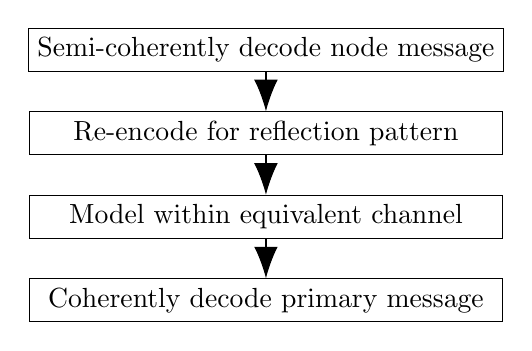
\begin{tikzpicture}[
		% every axis plot/.append style={thick},
		every node/.append style={draw,minimum width=6cm},
		align=center
	]
	\draw[-{Latex[length=4mm]}] (0,0) node[anchor=south](0){Semi-coherently decode node message} to ++(0,-0.5) node[anchor=north](1){Re-encode for reflection pattern};
	\draw[-{Latex[length=4mm]}] (1.south) to ++(0,-0.5) node[anchor=north](2){Model within equivalent channel};
	\draw[-{Latex[length=4mm]}] (2.south) to ++(0,-0.5) node[anchor=north](3){Coherently decode primary message};
\end{tikzpicture}

				}
			}
			\subfloat{
				\resizebox{0.58\linewidth}{!}{
					\input{../assets/viva/energy_distribution.tex}
				}
			}
			\label{fg:receiver}
		\end{figure}
		\vspace{0.5cm}
		\begin{itemize}
			\item Accumulated receive energy $z=\sum_{n} \bigl\lvert y[n] \bigr\rvert^2$ follows Gamma distribution
			\item \textcolor{orange}{Backscatter detection} under primary uncertainty is part of \textcolor{blue}{channel training}
			\item Requires one energy comparison and re-encoding per backscatter symbol (much simpler than symbiotic radio with $N$ \gls{sic} and 1 combining)
		\end{itemize}
	\end{frame}


	\begin{frame}{Joint beamforming, input distribution, and energy detector design}
		\vspace{-0.125cm}
		\begin{block}{Achievable rate}
			\vspace{-0.25cm}
			\begin{align*}
				\sum_k R_{\text{B},k} &= \sum\nolimits_{m_{\mathcal{K}}} P_{\mathcal{K}}(x_{m_{\mathcal{K}}}) \sum\nolimits_{m_{\mathcal{K}}'} P(\hat{x}_{m_{\mathcal{K}}'} \mid x_{m_{\mathcal{K}}}) \log {P(\hat{x}_{m_{\mathcal{K}}'} \mid x_{m_{\mathcal{K}}})}/{P(\hat{x}_{m_{\mathcal{K}}'})}\\
				R_{\text{P}} &= \sum\nolimits_{m_{\mathcal{K}}} P_{\mathcal{K}}(x_{m_{\mathcal{K}}}) N \log \left(1 + \frac{\lvert \mathbf{h}^\mathsf{H}(x_{m_{\mathcal{K}}}) \mathbf{w} \rvert^2}{\sigma_w^2}\right)
			\end{align*}
		\end{block}
		\begin{block}{Problem formulation}
			\vspace{-0.25cm}
			\begin{maxi*}
				{\scriptstyle{\{\mathbf{p}_k\},\mathbf{w},\mathbf{t}}}{\rho R_\text{P} + (1-\rho) \sum\nolimits_{k} R_{\text{B},k}}{}{}
				\addConstraint{\mathbf{1}^\mathsf{T} \mathbf{p}_k=1,}{\quad \mathbf{p}_k \ge \mathbf{0},}{\quad \forall k}
				\addConstraint{t_{l-1} \le t_l,}{\quad t_l \ge 0,}{\quad \forall l}
				\addConstraint{\lVert \mathbf{w} \rVert^2 \le P,}{}{}
			\end{maxi*}
		\end{block}
		\begin{exampleblock}{Solution by \gls{bcd}}
			\begin{itemize}
				\item Input distribution $\{\mathbf{p}_k\}$: \gls{kkt}
				\item Active beamforming $\mathbf{w}$: \gls{pga}
				\item Energy decision threshold $\mathbf{t}$: \gls{dp}
			\end{itemize}
		\end{exampleblock}
	\end{frame}

	\begin{frame}{Simulation results: Input distribution}
		\begin{figure}[!t]
			\centering
			\subfloat{
				\resizebox{0.48\linewidth}{!}{
					\input{../assets/viva/input_distribution.tex}
				}
			}
			\subfloat{
				\resizebox{0.48\linewidth}{!}{
					\input{../assets/viva/distribution_weights.tex}
				}
			}
		\end{figure}
		\begin{itemize}
			\item \gls{bc} and \gls{ris} are special cases of RIScatter with uniform and degenerate input distribution
			\item Increasing $\rho$ from 0 to 1 creates a smooth transition from backscatter modulation to passive beamforming
		\end{itemize}
	\end{frame}

	\begin{frame}{Simulation results: Rate region}
		\begin{figure}[!t]
			\centering
			\subfloat{
				\resizebox{0.48\linewidth}{!}{
					\input{../assets/viva/region_comparison.tex}
				}
			}
			\subfloat{
				\resizebox{0.48\linewidth}{!}{
					\input{../assets/viva/region_duration.tex}
				}
			}
		\end{figure}
		\begin{itemize}
			\item RIScatter backscatter rate is lower than symbiotic radio (due to energy detection) but higher than ambient backscatter (due to adaptive encoding)
			\item A large spreading factor $N$ improves backscatter \glsfmtshort{ber} but reduces data rate
			\item Active and passive transmission can share resource with mutual benefits
		\end{itemize}
	\end{frame}
\end{section}

\begin{section}{Shaping: \glsfmtshort{bd}-\glsfmtshort{ris} in \glsfmtshort{mimo}}
	\begin{frame}{Channel shaping using \glsfmtshort{ris}: From diagonal model to beyond}
		\begin{block}{Overview}
			\begin{itemize}\setlength\itemsep{20pt}
				\item \textit{What does this paper study?}

				To what extent can a passive \gls{ris} redistribute the singular values of a \gls{mimo} channel.
				\item \textit{How does it differ from previous work?}

				We consider a \gls{bd} architecture, depict the singular value region, derive analytical bounds, and solve the rate maximization problem.
				\item \textit{What are the benefits?}

				Channel shaping is ubiquitous for communication, sensing, and power transfer, which helps to decouple the \gls{ris}-transceiver design.
				We also propose an efficient and universal \gls{bd}-\gls{ris} design framework.
			\end{itemize}
		\end{block}
	\end{frame}

	\begin{frame}{Wave scattering model}
		\begin{block}{Diagonal \glsfmtshort{ris}}
			Each element acts as an individual scatterer with phase shift only
			\begin{equation*}
				\mathbf{\Theta} = \mathrm{diag}(\theta_1, \ldots, \theta_{N_\mathrm{S}}) = \mathrm{diag}(e^{\jmath \phi_1}, \ldots, e^{\jmath \phi_{N_\mathrm{S}}})
				%  =
				% \begin{bsmallmatrix}
				% 	\theta_1 & 0 & \cdots & 0 \\
				% 	0 & \theta_2 & \cdots & 0 \\
				% 	\vdots & \vdots & \ddots & \vdots \\
				% 	0 & 0 & \cdots & \theta_{N_\mathrm{S}}
				% \end{bsmallmatrix}
				\label{eq:diagonal_scattering_matrix}
			\end{equation*}
		\end{block}

		\begin{block}{\glsfmtshort{bd}-\glsfmtshort{ris}}
			Each group contains $L$ connected elements, allowing amplitude and phase control
			\vspace{-0.25cm}
			\begin{equation*}
				\mathbf{\Theta} = \mathrm{diag}(\mathbf{\Theta}_1,\ldots,\mathbf{\Theta}_G), \quad \mathbf{\Theta}_g^\mathsf{H} \mathbf{\Theta}_g = \mathbf{I}_L, \quad \forall g
				\label{eq:bd_ris}
			\end{equation*}
			\vspace{-0.5cm}
			\begin{itemize}
				\item \emph{Subchannel rearrangement:} allows each group to rearrange and combine the backward and forward subchannels by strength
				\vspace{-0.25cm}
				\begin{equation*}
					\sum_{n=1}^{N_\mathrm{S}} \lvert h_{\mathrm{B},n} \rvert \lvert h_{\mathrm{F},n} \rvert \to \sum_{g=1}^{G} \sum_{l=1}^{L} \lvert h_{\mathrm{B},\pi_{\mathrm{B},g}(l)} \rvert \lvert h_{\mathrm{F},\pi_{\mathrm{F},g}(l)} \rvert
					\vspace{-0.25cm}
				\end{equation*}
				\item \emph{Subspace alignment:} rotate backward-forward (intra-group, multiplicative) and direct-indirect (inter-group, additive) singular vectors
				\vspace{-0.25cm}
				\begin{equation*}
					\mathbf{H} = \overbrace{\mathbf{H}_\mathrm{D} + \sum_g \mathbf{U}_{\mathrm{B},g} \mathbf{\Sigma}_{\mathrm{B},g} \underbrace{\mathbf{V}_{\mathrm{B},g}^\mathsf{H} \mathbf{\Theta}_g \mathbf{U}_{\mathrm{F},g}}_\text{backward-forward} \mathbf{\Sigma}_{\mathrm{F},g} \mathbf{V}_{\mathrm{F},g}^\mathsf{H}}^\text{direct-indirect}
					\label{eq:channel_equivalent_svd}
				\end{equation*}
			\end{itemize}
		\end{block}
	\end{frame}

	\begin{frame}{Some concepts in differential geometry}
		The feasible domain of $\mathbf{\Theta}_g$ is a unitary Lie group $U(L)$ with Lie algebra $\mathfrak{u}(L)$.
		\vspace{0.25em}
		\begin{itemize}
			\item \emph{Geodesic:} shortest path between two points on a manifold
			\item \emph{Lie group:} a group that is also a differentiable manifold
			\item \emph{Lie algebra:} tangent space of Lie group at the identity element
			% \item \emph{Exponential map:} maps the Lie algebra to the Lie group
		\end{itemize}
		\begin{figure}
			\centering
			\includegraphics[width=0.65\textwidth]{../assets/viva/lie_group.pdf}
		\end{figure}
		A geodesic emanating from the identity with velocity $\mathbf{D} \in \mathfrak{u}(L)$ can be described by the exponential map
		\begin{equation*}
			\mathbf{G}_\mathbf{I}(\mu) = \exp(\mu \mathbf{D})
			\label{eq:geodesic_identity}
		\end{equation*}

	\end{frame}

	\begin{frame}{Geodesic \glsfmtshort{rcg} via Lie algebra}
		\begin{block}{Non-geodesic vs geodesic \gls{rcg}}
			\begin{itemize}
				\item Non-geodesic: add then retract
				\begin{equation*}
					\bar{\mathbf{\Theta}}_g^{(r+1)} = \mathbf{\Theta}_g^{(r)} + \mu \mathbf{D}_g^{(r)}, \quad \mathbf{\Theta}_g^{(r+1)} = \bar{\mathbf{\Theta}}_g^{(r+1)} \bigl({\bar{\mathbf{\Theta}}_g^{(r+1)\mathsf{H}}} \bar{\mathbf{\Theta}}_g^{(r+1)}\bigr)^{-1/2}
				\end{equation*}
				\item Geodesic: multiplicative and rotational update
				\begin{equation*}
					\mathbf{\Theta}_g^{(r+1)} = \mathbf{G}_g^{(r)}(\mu) = \exp(\mu \mathbf{D}_g^{(r)}) \mathbf{\Theta}_g^{(r)}
					\label{eq:update_geodesic}
				\end{equation*}
			\end{itemize}
		\end{block}
		\begin{exampleblock}{Performance comparison}
			\begin{table}
				\label{tb:complexity_test}
				\centering
				\tiny
				\begin{tabular}{ccccccc}
					\toprule
					\multirow{2}{*}{\gls{rcg} path} & \multicolumn{3}{c}{$N_\mathrm{S}=16$} & \multicolumn{3}{c}{$N_\mathrm{S}=256$}                                                               \\ \cmidrule(lr){2-4} \cmidrule(lr){5-7}
													& Objective                             & Iterations                             & Time [s]         & Objective        & Iterations & Time [s] \\ \midrule
					Geodesic                        & $\num{4.359e-3}$                      & 11.59                                  & $\num{1.839e-2}$ & $\num{1.163e-2}$ & 25.58      & 3.461    \\
					Non-geodesic                    & $\num{4.329e-3}$                      & 30.92                                  & $\num{5.743e-2}$ & $\num{1.116e-2}$ & 61.40      & 13.50    \\ \bottomrule
				\end{tabular}
			\end{table}
		\end{exampleblock}
	\end{frame}

	\begin{frame}{Singular value redistribution: Optimization approach}
		\begin{block}{Pareto frontier of singular values}
			\begin{maxi*}
				{\scriptstyle{\mathbf{\Theta}}}{\sum_n \rho_n \sigma_n(\mathbf{H})}{}{}
				\addConstraint{\mathbf{\Theta}_g^\mathsf{H} \mathbf{\Theta}_g=\mathbf{I},}{\quad \forall g,}{}
			\end{maxi*}
		\end{block}
		\begin{exampleblock}{Solution by group-wise geodesic \glsfmtshort{rcg}}
			\begin{itemize}
				\item Faster convergence thanks to appropriate parameter space
				\item Step size $\mu$ can be obtained by the Armijo rule
				\item Doubling $\mu$ is computationally efficient $\exp(2 \mu \mathbf{D}_g^{(r)}) = \exp^2(\mu \mathbf{D}_g^{(r)})$
			\end{itemize}
		\end{exampleblock}
	\end{frame}

	\begin{frame}{Singular value redistribution: Analysis approach}
		\fontsize{6pt}{7.2}\selectfont
		\begin{proposition}[Degree of freedom]\label{pp:dof}
			In point-to-point \gls{mimo}, \gls{bd}-\gls{ris} cannot achieve a higher \gls{dof} than diagonal \gls{ris}.
		\end{proposition}
		\begin{proposition}[Rank-deficient channel]\label{pp:rank_deficient}
			If the forward or backward channel is rank-$k$ ($k \le N$), then regardless of the passive \gls{ris} size and architecture, the $n$-th singular value of the equivalent channel is bounded by
			\begin{align*}
				\sigma_n(\mathbf{H}) & \le \sigma_{n-k}(\mathbf{T}), &  & \text{if } n > k,         \\
				\sigma_n(\mathbf{H}) & \ge \sigma_n(\mathbf{T}),     &  & \text{if } n < N - k + 1,
			\end{align*}
			where
			\begin{equation*}
				\mathbf{T} \mathbf{T}^\mathsf{H} =
				\begin{cases}
					\mathbf{H}_\mathrm{D} (\mathbf{I} - \mathbf{V}_\mathrm{F} \mathbf{V}_\mathrm{F}^\mathsf{H}) \mathbf{H}_\mathrm{D}^\mathsf{H}, & \text{if } \mathrm{rank}(\mathbf{H}_\mathrm{F}) = k, \\
					\mathbf{H}_\mathrm{D}^\mathsf{H} (\mathbf{I} - \mathbf{U}_\mathrm{B} \mathbf{U}_\mathrm{B}^\mathsf{H}) \mathbf{H}_\mathrm{D}, & \text{if } \mathrm{rank}(\mathbf{H}_\mathrm{B}) = k,
				\end{cases}
				\label{eq:auxiliary_matrix}
			\end{equation*}
			and $\mathbf{V}_\mathrm{F}$ and $\mathbf{U}_\mathrm{B}$ are the right and left compact singular matrices of $\mathbf{H}_\mathrm{F}$ and $\mathbf{H}_\mathrm{B}$, respectively.
		\end{proposition}
		\begin{proposition}[Unitary \gls{ris} without direct link]\label{pp:fully_connected}
			If the \gls{bd}-\gls{ris} is unitary and the direct link is absent, then the channel singular values can be manipulated up to
			\begin{equation*}
				\mathrm{sv}(\mathbf{H}) = \mathrm{sv}(\mathbf{BF}),
			\end{equation*}
			where $\mathbf{B}$ and $\mathbf{F}$ are arbitrary matrices with the same singular values as $\mathbf{H}_\mathrm{B}$ and $\mathbf{H}_\mathrm{F}$, respectively,
		\end{proposition}
	\end{frame}

	\begin{frame}{Achievable rate maximization}
		\begin{block}{Problem formulation}
			\begin{maxi*}
				{\scriptstyle{\mathbf{W},\mathbf{\Theta}}}{R = \log \det \biggl(\mathbf{I} + \frac{\mathbf{W}^\mathsf{H}\mathbf{H}^\mathsf{H}\mathbf{H}\mathbf{W}}{\eta}\biggr)}{}{}
				\addConstraint{\lVert \mathbf{W} \rVert _\mathrm{F}^2}{\le P}
				\addConstraint{\mathbf{\Theta}_g^\mathsf{H} \mathbf{\Theta}_g}{=\mathbf{I}, \quad \forall g.}
			\end{maxi*}
		\end{block}
		\begin{exampleblock}{Local-optimal solution: \gls{bcd}}
			\begin{itemize}
				\item Passive beamforming $\mathbf{\Theta}$: group-wise geodesic \gls{rcg}
				\item Active beamforming $\mathbf{W}$: eigenmode transmission and water-filling
			\end{itemize}
		\end{exampleblock}
		\begin{exampleblock}{Low-complexity solution: two-stage}
			\begin{itemize}
				\item Shaping stage: channel power gain maximization, solved in closed form
				\item Transmission stage: eigenmode transmission and water-filling
			\end{itemize}
		\end{exampleblock}
	\end{frame}

	\begin{frame}{Simulation results: Singular value}
		\begin{figure}
			\centering
			\subfloat[$2 \times 32 \times 2$\label{fg:singular_pareto_sx32}]{
				\resizebox{!}{3cm}{
					\input{../assets/viva/singular_pareto_sx32.tex}
				}
			}
			\subfloat[$2 \times 128 \times 2$\label{fg:singular_pareto_sx128}]{
				\resizebox{!}{3cm}{
					\input{../assets/viva/singular_pareto_sx128.tex}
				}
			}
			\subfloat[$4 \times 32 \times 4$ (rank-1)\label{fg:singular_bound_rank2_sx128}]{
				\resizebox{!}{3cm}{
					\input{../assets/viva/singular_bound_rank2_sx128.tex}
				}
			}
			\label{fg:singular_bound}
		\end{figure}
		\vspace{1em}
		\begin{itemize}
			\item \gls{bd}-\gls{ris} provides \qty{22}{\percent} and \qty{38}{\percent} dynamic range gain for $\sigma_1(\mathbf{H})$ and $\sigma_2(\mathbf{H})$
			\item Increasing group size enlarges singular value region with better trade-off
			\item Asymptotic bounds in rank-deficient channels are valid for both architectures
		\end{itemize}
	\end{frame}

	\begin{frame}{Simulation results: Achievable rate}
		\begin{figure}
			\centering
			\subfloat[$4 \times 128 \times 4$\label{fg:rate_beamforming}]{
				\resizebox{!}{2.9cm}{
					\input{../assets/viva/rate_beamforming.tex}
				}
			}
			\subfloat[$N_\mathrm{T} \times 128 \times N_\mathrm{R}$\label{fg:rate_txrx}]{
				\resizebox{!}{2.9cm}{
					\input{../assets/viva/rate_txrx.tex}
				}
			}
			\subfloat[$4 \times N_\mathrm{S} \times 4$\label{fg:rate_sx}]{
				\resizebox{!}{2.9cm}{
					\input{../assets/viva/rate_sx.tex}
				}
			}
			\label{fg:rate}
		\end{figure}
		\vspace{1em}
		\begin{itemize}
			\item Deficit from low-complexity design vanishes as \gls{ris} evolves towards unitary
			\item \gls{bd}-\gls{ris} can activate multiple streams at lower transmit power
			\item Percentage rate gain of \gls{bd}-\gls{ris} scales with \gls{mimo} dimension and group size
		\end{itemize}
	\end{frame}
\end{section}

\begin{section}{Outro}
	\begin{frame}{Future works: I}
		\begin{block}{Coherent RIScatter detector}
			\begin{equation*}
				y[n] = {\mathbf{h}_{\text{D}}^\mathsf{H} + \mathbf{h}_{\text{C}}^\mathsf{H} {x}} \mathbf{w} {s[n]} + v[n],
			\end{equation*}
			\begin{itemize}
				\item Same model as index modulation
				\item $x$ has finite support $\to$ $y[n]$ is a Gaussian mixture (non-elementary entropy)
				\item Achievable rate can be approximated as
				\begin{equation*}
					R_\text{B} = \sum_i p(x_i) \log \sum_j p(x_j) \frac{4 \sigma_i^2 \sigma_j^2}{(\sigma_i^2 + \sigma_j^2)^2}
				\end{equation*}
				\item \gls{ber} performance?
				\item Code-domain \gls{noma}?
			\end{itemize}
		\end{block}
	\end{frame}

	\begin{frame}{Future works: II}
		\begin{block}{Multiplicative broadcast channel}
			The received signal is
			\begin{equation*}
				y_k = h_k \prod_q x_q + n.
			\end{equation*}
			\begin{itemize}
				\item \gls{sic} $\to$ successive channel refinement (better symbol-level precoding)
				\item \textcolor{blue}{Log-normal} is also maximum entropy distribution
				\item Product of log-normal is log-normal
			\end{itemize}
		\end{block}

		\begin{exampleblock}{Index modulation is a special case with superuser $R = R_1 + R_2$}
			\begin{itemize}
				\item $x_1 \sim \mathcal{CN}(0, \sigma_1^2)$ and $x_2$ with finite support
				\item Index message encoded in the Euclidean distance between $h x_2^{(i)}$
				\item Decode $x_2$ first, rate depends on {entropy of Gaussian mixture}
			\end{itemize}
		\end{exampleblock}
	\end{frame}

	\begin{frame}{Future works: III}
		\begin{block}{Rate splitting $\times$ index modulation}
			The received signal is
			\begin{equation*}
				y_k = h_k \theta \sum_q x_q + n.
			\end{equation*}
			\vspace{-1em}
			\begin{itemize}
				\item Dynamic \gls{ris} achieves the convex hull below by time-sharing \cite{Mu2021a}
				\begin{figure}
					\centering
					\subfloat{
						\resizebox{0.4\columnwidth}{!}{
							\includegraphics[scale=1]{../assets/viva/rate_region_noma.jpg}
						}
					}
					\subfloat{
						\resizebox{0.4\columnwidth}{!}{
							\includegraphics[scale=1]{../assets/viva/rate_region_oma.jpg}
						}
					}
				\end{figure}
				\item Common message can be embedded in $\theta$ to push the boundary
			\end{itemize}
		\end{block}
	\end{frame}

	\begin{frame}{Future works: III}
		\begin{block}{Feasibility of interference alignment by \gls{ris}}
			\begin{align*}
				&\text{find} && \mathbf{\Theta} &&&\\
				&\text{s.t.} && \mathbf{H}^{[kj]} = \mathbf{H}_\mathrm{D}^{[kj]} + \mathbf{H}_\mathrm{B}^{[k]} \mathbf{\Theta} \mathbf{H}_\mathrm{F}^{[j]} = \mathbf{0}, &&& \forall j \neq k\\
				& && \mathrm{rank}(\mathbf{H}^{[kk]}) = d_k, &&& \forall k
			\end{align*}
			\begin{itemize}
				\item Necessary and sufficient feasibility conditions?
				\item How many scattering elements are required on expectation?
				\item Multi-sector \gls{bd}-\gls{ris} \cite{Li2023c}?
			\end{itemize}
		\end{block}
	\end{frame}

\end{section}
% \end{section}

% \begin{section}{Research Proposal}
% 	\begin{subsection}{STAR-RIS: Interference Alignment}
% 		\begin{frame}{STAR-RIS in Interference Channel (I)}
% 			Consider a STAR-RIS-aided interference \gls{mimo} of $K$ transmitter-receiver pairs.
% 			\begin{block}{Leakage interference minimization}
% 				\vspace{-2em}
% 				\begin{mini!}
% 					{\scriptstyle{\mathbf{\Theta}, \{\mathbf{G}_k\}, \{\mathbf{W}_k\}}}{\mathop{\sum\sum}_{j \neq k} \bigl\lVert \mathbf{G}_k \underbrace{(\mathbf{H}^{[kj]}_\mathrm{D} + \mathbf{H}^{[k]}_\mathrm{B} \mathbf{\Theta}^{[kj]} \mathbf{H}^{[j]}_{\mathrm{F}})}_{\triangleq \mathbf{H}^{[kj]}} \mathbf{W}_j \bigr\rVert _{\mathrm{F}}^2}{\label{op:leakage}}{}
% 					\addConstraint{\mathbf{\Theta}_{\mathrm{T},g}^\mathsf{H} \mathbf{\Theta}_{\mathrm{T},g}+\mathbf{\Theta}_{\mathrm{R},g}^\mathsf{H} \mathbf{\Theta}_{\mathrm{R},g}=\mathbf{I}, \quad}{\forall g}{\label{co:scatter}}
% 					\addConstraint{\mathbf{G}_k \mathbf{G}_k^\mathsf{H}=\mathbf{I}, \quad}{\forall k}{\label{co:combiner}}
% 					\addConstraint{\mathbf{W}_j^\mathsf{H} \mathbf{W}_j=\mathbf{I}, \quad}{\forall j,}{\label{co:precoder}}
% 				\end{mini!}
% 			\end{block}

% 			\begin{block}{Feasibility of interference alignment}
% 				\vspace{-1em}
% 				\begin{subequations}
% 					\begin{align}
% 						&\text{find} && \mathbf{\Theta}, \{\mathbf{G}_k\}, \{\mathbf{W}_k\} &&&\\
% 						&\text{s.t.} && \mathbf{G}_k \mathbf{H}^{[kj]} \mathbf{W}_j = \mathbf{0}, &&& \forall j \neq k\\
% 						& && \mathrm{rank}(\mathbf{G}_k \mathbf{H}^{[kk]} \mathbf{W}_k) = d_k, &&& \forall k
% 					\end{align}
% 				\end{subequations}
% 			\end{block}
% 		\end{frame}

% 		\begin{frame}{STAR-RIS in Interference Channel (II)}
% 			\begin{block}{Weighted sum-rate maximization}
% 				\vspace{-2em}
% 				\begin{maxi!}
% 					{\scriptstyle{\mathbf{\Theta}, \{\mathbf{W}_k\}}}{\sum_k \rho_k \log \det \biggl(\mathbf{I} + \mathbf{W}_k {\mathbf{H}^{[kj]}}^\mathsf{H} \mathbf{Q}_k^{-1} {\mathbf{H}^{[kj]}} \mathbf{W}_k\biggr)}{\label{op:ic_rate}}{\label{ob:ic_rate}}
% 					\addConstraint{\mathbf{\Theta}_{\mathrm{T},g}^\mathsf{H} \mathbf{\Theta}_{\mathrm{T},g}+\mathbf{\Theta}_{\mathrm{R},g}^\mathsf{H} \mathbf{\Theta}_{\mathrm{R},g}=\mathbf{I}, \quad}{\forall g}{}
% 					\addConstraint{\lVert \mathbf{W}_k \rVert _\mathrm{F}^2 \le P_k, \quad}{\forall k,}{}
% 				\end{maxi!}
% 				where $\mathbf{Q}_k$ is the interference-plus-noise covariance matrix at receiver $k$
% 				\begin{equation*}
% 					\mathbf{Q}_k = \sum_{j \ne k} {\mathbf{H}^{[kj]}} \mathbf{W}_j {\mathbf{W}_j}^\mathsf{H} {\mathbf{H}^{[kj]}}^\mathsf{H} + \eta \mathbf{I},
% 				\end{equation*}
% 			\end{block}
% 		\end{frame}
% 	\end{subsection}

% 	\begin{subsection}{NOMA: Index Modulation}
% 		\begin{frame}{\glsfmtlong{im} is a Multiplicative NOMA}
% 			\begin{block}{Multiplicative broadcast channel}
% 				The received signal is
% 				\begin{equation*}
% 					y_k = h_k \prod_q x_q + n.
% 				\end{equation*}
% 				\begin{itemize}
% 					\item \gls{sic} $\to$ successive channel refinement (better symbol-level precoding)
% 					\item \textcolor{blue}{Log-normal} is also maximum entropy distribution
% 					\item Product of log-normal is log-normal
% 				\end{itemize}
% 			\end{block}

% 			\begin{exampleblock}{Index modulation is a special case with superuser $R = R_1 + R_2$}
% 				\begin{itemize}
% 					\item $x_1 \sim \mathcal{CN}(0, \sigma_1^2)$ and $x_2$ with finite support
% 					\item Index message encoded in the Euclidean distance between $h x_2^{(i)}$
% 					\item Decode $x_2$ first, rate depends on \textcolor{blue}{entropy of Gaussian mixture}
% 				\end{itemize}
% 			\end{exampleblock}
% 		\end{frame}

% 		\begin{frame}{Multiplicative NOMA: Another Example}
% 			\begin{block}{Joint transmitter-\gls{ris} encoding}
% 				The received signal is
% 				\begin{equation*}
% 					y_k = h_k \theta \sum_q x_q + n.
% 				\end{equation*}
% 				\vspace{-1em}
% 				\begin{itemize}
% 					\item Dynamic \gls{ris} can achieve the convex hull of static \gls{ris} \cite{Mu2021a}
% 					\begin{figure}
% 						\centering
% 						\subfloat{
% 							\resizebox{0.4\columnwidth}{!}{
% 								\includegraphics[scale=1]{assets/rate_region_noma.jpg}
% 							}
% 						}
% 						\subfloat{
% 							\resizebox{0.4\columnwidth}{!}{
% 								\includegraphics[scale=1]{assets/rate_region_oma.jpg}
% 							}
% 						}
% 					\end{figure}
% 					\item Joint encoding rides additional information on $\theta$ as ``common message''
% 				\end{itemize}
% 			\end{block}
% 		\end{frame}
% 		\begin{frame}{Thank You}
% 			\begin{figure}
% 				\centering
% 				\includegraphics[width=0.8\columnwidth]{assets/ris.jpg}
% 			\end{figure}
% 		\end{frame}
% 	\end{subsection}
% \end{section}

\bibliographystyle{IEEEtran}
\bibliography{../misc/library.bib}
\end{document}
